\documentclass{protokol}

\usepackage[czech]{babel}
\usepackage[utf8]{inputenc}
\usepackage{icomma}

% Plovouci bloky (obrazky, tabulky)
\usepackage{floatrow}
\floatsetup[table]{capposition=top}
\floatsetup[figure]{frameset={\fboxsep16pt}}
\usepackage{subcaption}

% Tabulky
\usepackage{tabu}
\usepackage{booktabs}
\usepackage{csvsimple}
\usepackage{multirow}
\usepackage{multicol}

% Jednotky
\usepackage{siunitx}
\sisetup{
	locale               = DE,
	inter-unit-product   = \ensuremath{{}\cdot{}},
	list-units           = single,
	list-separator       = {; },
	list-final-separator = \text{ a },
	list-pair-separator  = \text{ a },
	range-phrase         = \text{ až },
	range-units          = single,
}
\usepackage{amsmath}

% Obvody
\usepackage{circuitikz}

% Obrazky a grafy
% \usepackage{graphicx}
\graphicspath{
	{plots/}
	{build/plots/}
	{img/}
}
\usepackage{epstopdf}
\epstopdfsetup{outdir=./build/plots/}

\jmenopraktika={Experimentální metody}
\jmeno={Radek Horňák, Jan Slaný, Lukáš Vrána}
\obor={Fyzika plazmatu}
\skupina={Pá 8:00}
\rocnik={IV}
\semestr={VIII}

\cisloulohy={}
\jmenoulohy={Měření povrchové energie}

\datum={17. května 2022}
\tlak={}% [hPa]
\teplota={}% [C]
\vlhkost={}% [%]

\begin{document}
\header
\section{Úvod}
\par Povrchová energie je práce $W$, kterou je potřeba vykonat pro vznik 
jednotky plochy $A$:
\begin{equation}
	W = \gamma\Delta A
\end{equation}
Na rozhraní pevné látky, kapaliny a plynu jsou přítomná tři povrchová napětí: 
$\gamma_{\text{sv}}$ je povrchové napětí mezi pevnou látkou a párou, 
$\gamma_{\text{lv}}$ je 
povrchové napětí mezi kapalinou a párou, $\gamma_{\text{sl}}$ je povrchové 
napětí 
mezi pevnou látkou a kapalinou. Kontaktní úhel $\theta$ je úhel měřený 
v~kapalině na tomto rozhraní, viz~obr.~\ref{wetting}. 
\begin{figure}[b]
	\begin{center}
		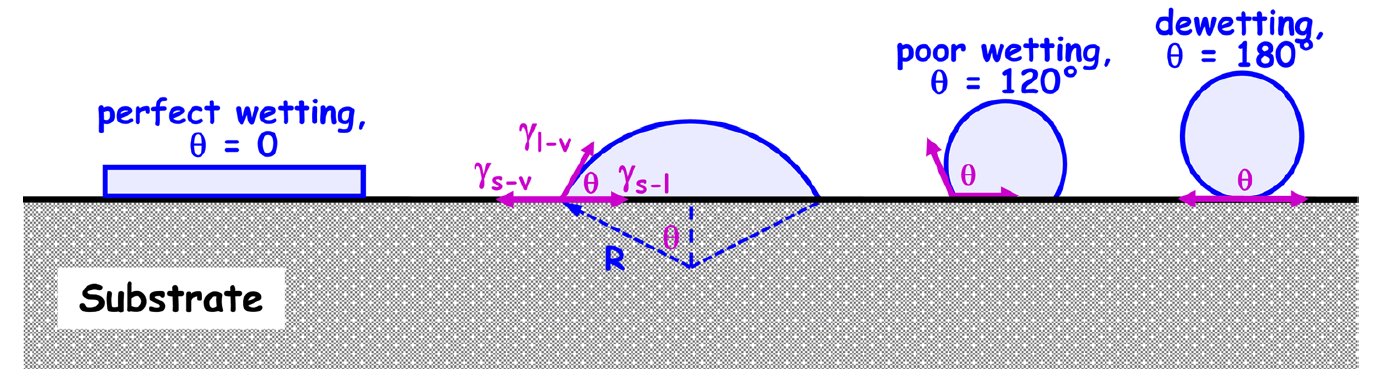
\includegraphics[width=\textwidth]{wetting.png}
		\captionof{figure}{Ilustrace povrchového napětí $\gamma$ a kontaktního 
		úhlu $\theta$.}
		\label{wetting}
	\end{center} 
\end{figure}
\par Povrchová energie materiálu je úměrná přilnavosti či fixaci na daný 
povrch. V praxi to znamená, že požadujeme vysokou povrchovou energii pro dobrou 
adhezi tiskařské barvy, lepidel, laků či nátěrů. Nízká povrchová energie je 
užitečná např. u skel na autě nebo u kuchyňského nádobí (pánví). Povrchová 
energie je vlastností materiálu, ale také jeho znečištěním, 
např. otisky prstů mohou snížit povrchovou energii.
\par Existuje několik metod, jak povrchovou energii určit. Nejjednodušší jsou 
fixy, které jsou kalibrované pro danou hodnotu povrchové energie. Pokud fix 
zanechá na povrchu malé kapičky, znamená to, že povrch má nižší povrchovou 
energii než je uvedená hodnota na fixu. Tato metoda se nejčastěji užívá v~průmyslu, kde požadujeme, aby výrobek měl nižší (nebo vyšší) povrchovou energii 
než daná hodnota. Podobnou metodou jsou testovací inkousty. Jejich princip je 
stejný jako u fixů, kapalinu nanášíme štětečkem na povrch. Fixy ani inkousty 
nepotřebují přívod elektřiny či počítač, jsou ale drahé a mají krátkou 
životnost (3 až 6 měsíců).
\par Kapková metoda je založena na sledování tvaru kapky testovací kapaliny 
usazené na povrchu vzorku. Testovací kapaliny nesmí reagovat se vzorkem, musí 
mít známé a stálé parametry, neměly by být toxické, nesmí se rychle vypařovat a 
jejich povrchové napětí musí být vyšší než povrchová energie pevné látky. 
Výhodou této metody je určení hodnoty povrchové energie včetně chybové analýzy 
dle použitých modelů. Mezi chyby měření patří špatně usazená kapka, špatný fit 
profilu kapky, nehomogenita vzorku, sejmutí profilu před dosažením 
termodynamické rovnováhy, kontaminace měřicích kapalin~aj.

\section{Praktická část}
\subsection{Měření kontaktního úhlu}
\par Pro měření povrchové energie byl použit přístroj See System, který můžeme vidět na 
obr.~\ref{ss}. Přístroj je složen ze stolku o~velikosti $10 \times 10$~cm, 
který lze dvěma stavěcími šrouby posouvat do všech směrů, a 2Mpix kamery, která 
snímá povrch. Na stolek se položí substrát, jehož povrchovou energii chceme 
zkoumat. Mikropipetou se nanese na povrch kapka a stolek se stavěcími šrouby 
naladí tak, aby kamera ostře snímala kapku na povrchu. Přístroj je připojen USB 
portem k~počítači, který pomocí příslušného softwaru dokáže ovládat kameru. 
Jakmile je kapka ostře vidět, přes software uložíme fotku z~kamery a dále 
zpracujeme. Na kapce zvolíme ručně tři body -- dvě na rozhraní pevná látka -- 
kapalina -- plyn a třetí bod na vrcholu kapky, čímž určíme kontaktní úhel pro 
danou testovací kapalinu, viz obr.~\ref{ssw}. Pokud toto uděláme pro kapky 
alespoň dvou různých kapalin, software dokáže spočítat povrchovou energii 
pomocí běžných modelů. 
\par Měřili jsme povrchovou energii teflonu. Před měřením jsme povrch očistili 
isopropylalkoholem. Následně jsme měřili kontaktní úhel šesti testovacích 
kapalin: voda, etylenglykol, dijodometan, glycerol, formamid, 
$\alpha$-bromnaftalen. U každé kapaliny jsme naměřili kontaktní úhel 10 
kapek, viz tabulka~\ref{table:surfTensionLiquid}. Pro výpočet povrchové 
energie jsme použili několik metod, které se liší svou komplikovaností, ale 
také určením pro dané povrchy.

\begin{figure}[h]
	\begin{center}
		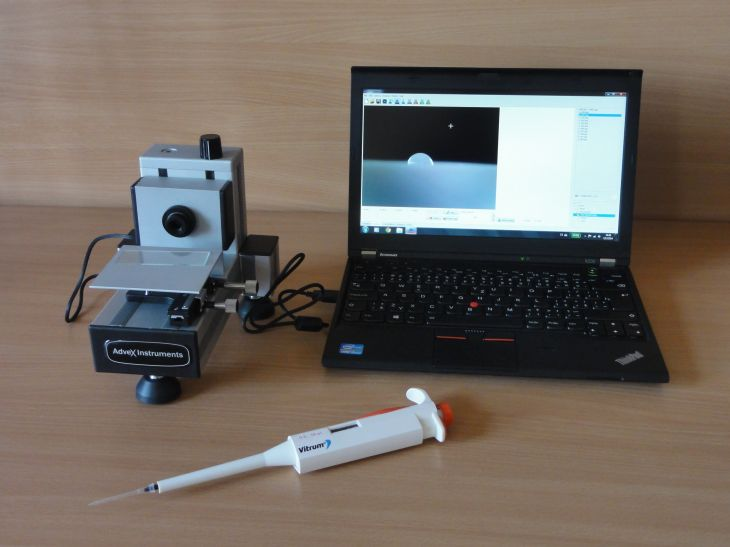
\includegraphics[width=0.9\textwidth]{seesystem.jpg}
		\captionof{figure}{Přístroj See System pro měření kontaktního úhlu 
		kapky a určení povrchové energie.}
		\label{ss}
	\end{center} 
\end{figure}

\begin{figure}
	\begin{center}
		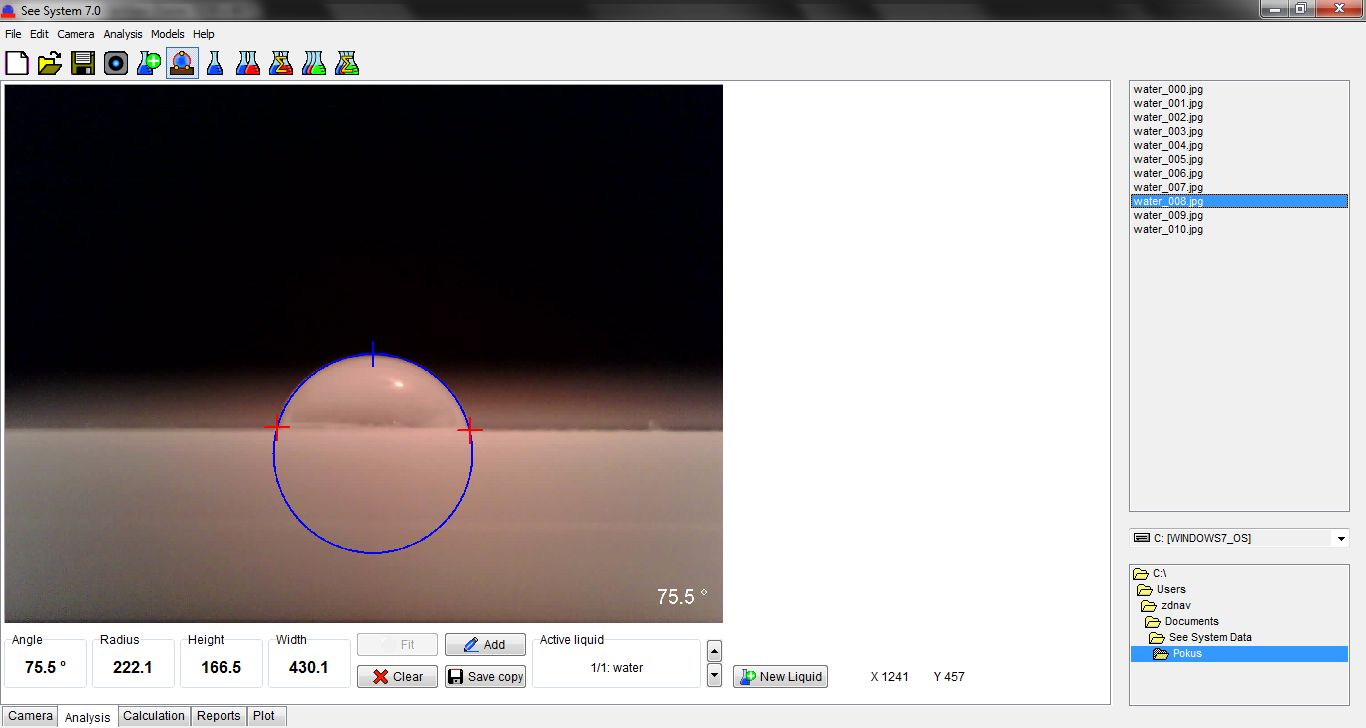
\includegraphics[width=\textwidth]{seesystemsw.jpg}
		\captionof{figure}{Ukázka tříbodového určení kontaktního úhlu pomocí 
		See System softwaru.}
		\label{ssw}
	\end{center} 
\end{figure}


\subsection{Zismanova metoda}
\par Zismanova metoda je založena na vynesení závislosti $\cos\theta = 
f\left(\gamma_{\text{l}} \right)$ do grafu. Po naměření kontaktních úhlů 
$\theta$ pro několik kapalin se známou hodnotou povrchové energie 
$\gamma_{\text{l}}$ (tab.~\ref{table:surfTensionLiquid}) můžeme fitovat 
závislost rovnicí
\begin{equation}
	\cos\theta = 1 + 
	b \left( \gamma_{\text{c}} - \gamma_{\text{l}} \right)
\end{equation}
ze které získáme hodnotu celkové povrchové energie $\gamma_{\text{c}}$. Tento 
fit jsme pro ukázku provedli na obr.~\ref{graph:zisman}. Z fitu jsme vyřadili 
etylenglykol, jelikož jeho ponechání vedlo k nesmyslným hodnotám. Ze závislosti 
určená celková povrchová energie je $\gamma_{\text{c}} = 
(4,5\pm11,5)$\,\si{\milli\joule\per\meter\squared}. Software měřicího přístroje určil 
$\gamma_{\text{c}}~=~(5,7~\pm~16,9)$~\si{\milli\joule\per\meter\squared}. Z chyb měření lze vidět, že 
tato 
metoda není pro určení povrchové energie teflonu vhodná.

\begin{table}[h]
	\caption{Naměřený kontaktní úhel $\theta$ a tabelované povrchové napětí 
		$\gamma_{\text{l}}$ testovacích kapalin \cite{napetiKapalin}.}
	\label{table:surfTensionLiquid}
	\begin{tabular}{|c|c|c|}\hline
		kapalina  & Kontaktní úhel $\theta$\,[\si{\deg}] &
		$\gamma_{\text{l}}$\,[\si{\milli\joule\per\meter\squared}]\\ \hline
		destilovaná voda & $102\pm4$ & 72,8                              \\
		etylenglykol     & $88\pm4$ & 47,7                              \\
		dijodometan      & $77\pm4$ & 50,8                              \\
		glycerol         & $99\pm6$ & 64,0                              \\
		formamid         & $91\pm2$ & 58,2                              \\
		$\alpha$-bromnaftalen &$68\pm3$ & 44,4  \\ \hline
	\end{tabular}
\end{table}

%HODNOTY $\gamma_{\text{l}}$
%https://en.wikipedia.org/wiki/Surface-tension_values 
%https://en.wikipedia.org/wiki/Glycerol_(data_page)
%https://pubchem.ncbi.nlm.nih.gov/compound/formamide#section=Heat-of-Vaporization
%http://www.surface-tension.de/

\begin{figure}[h!]
	\centering
	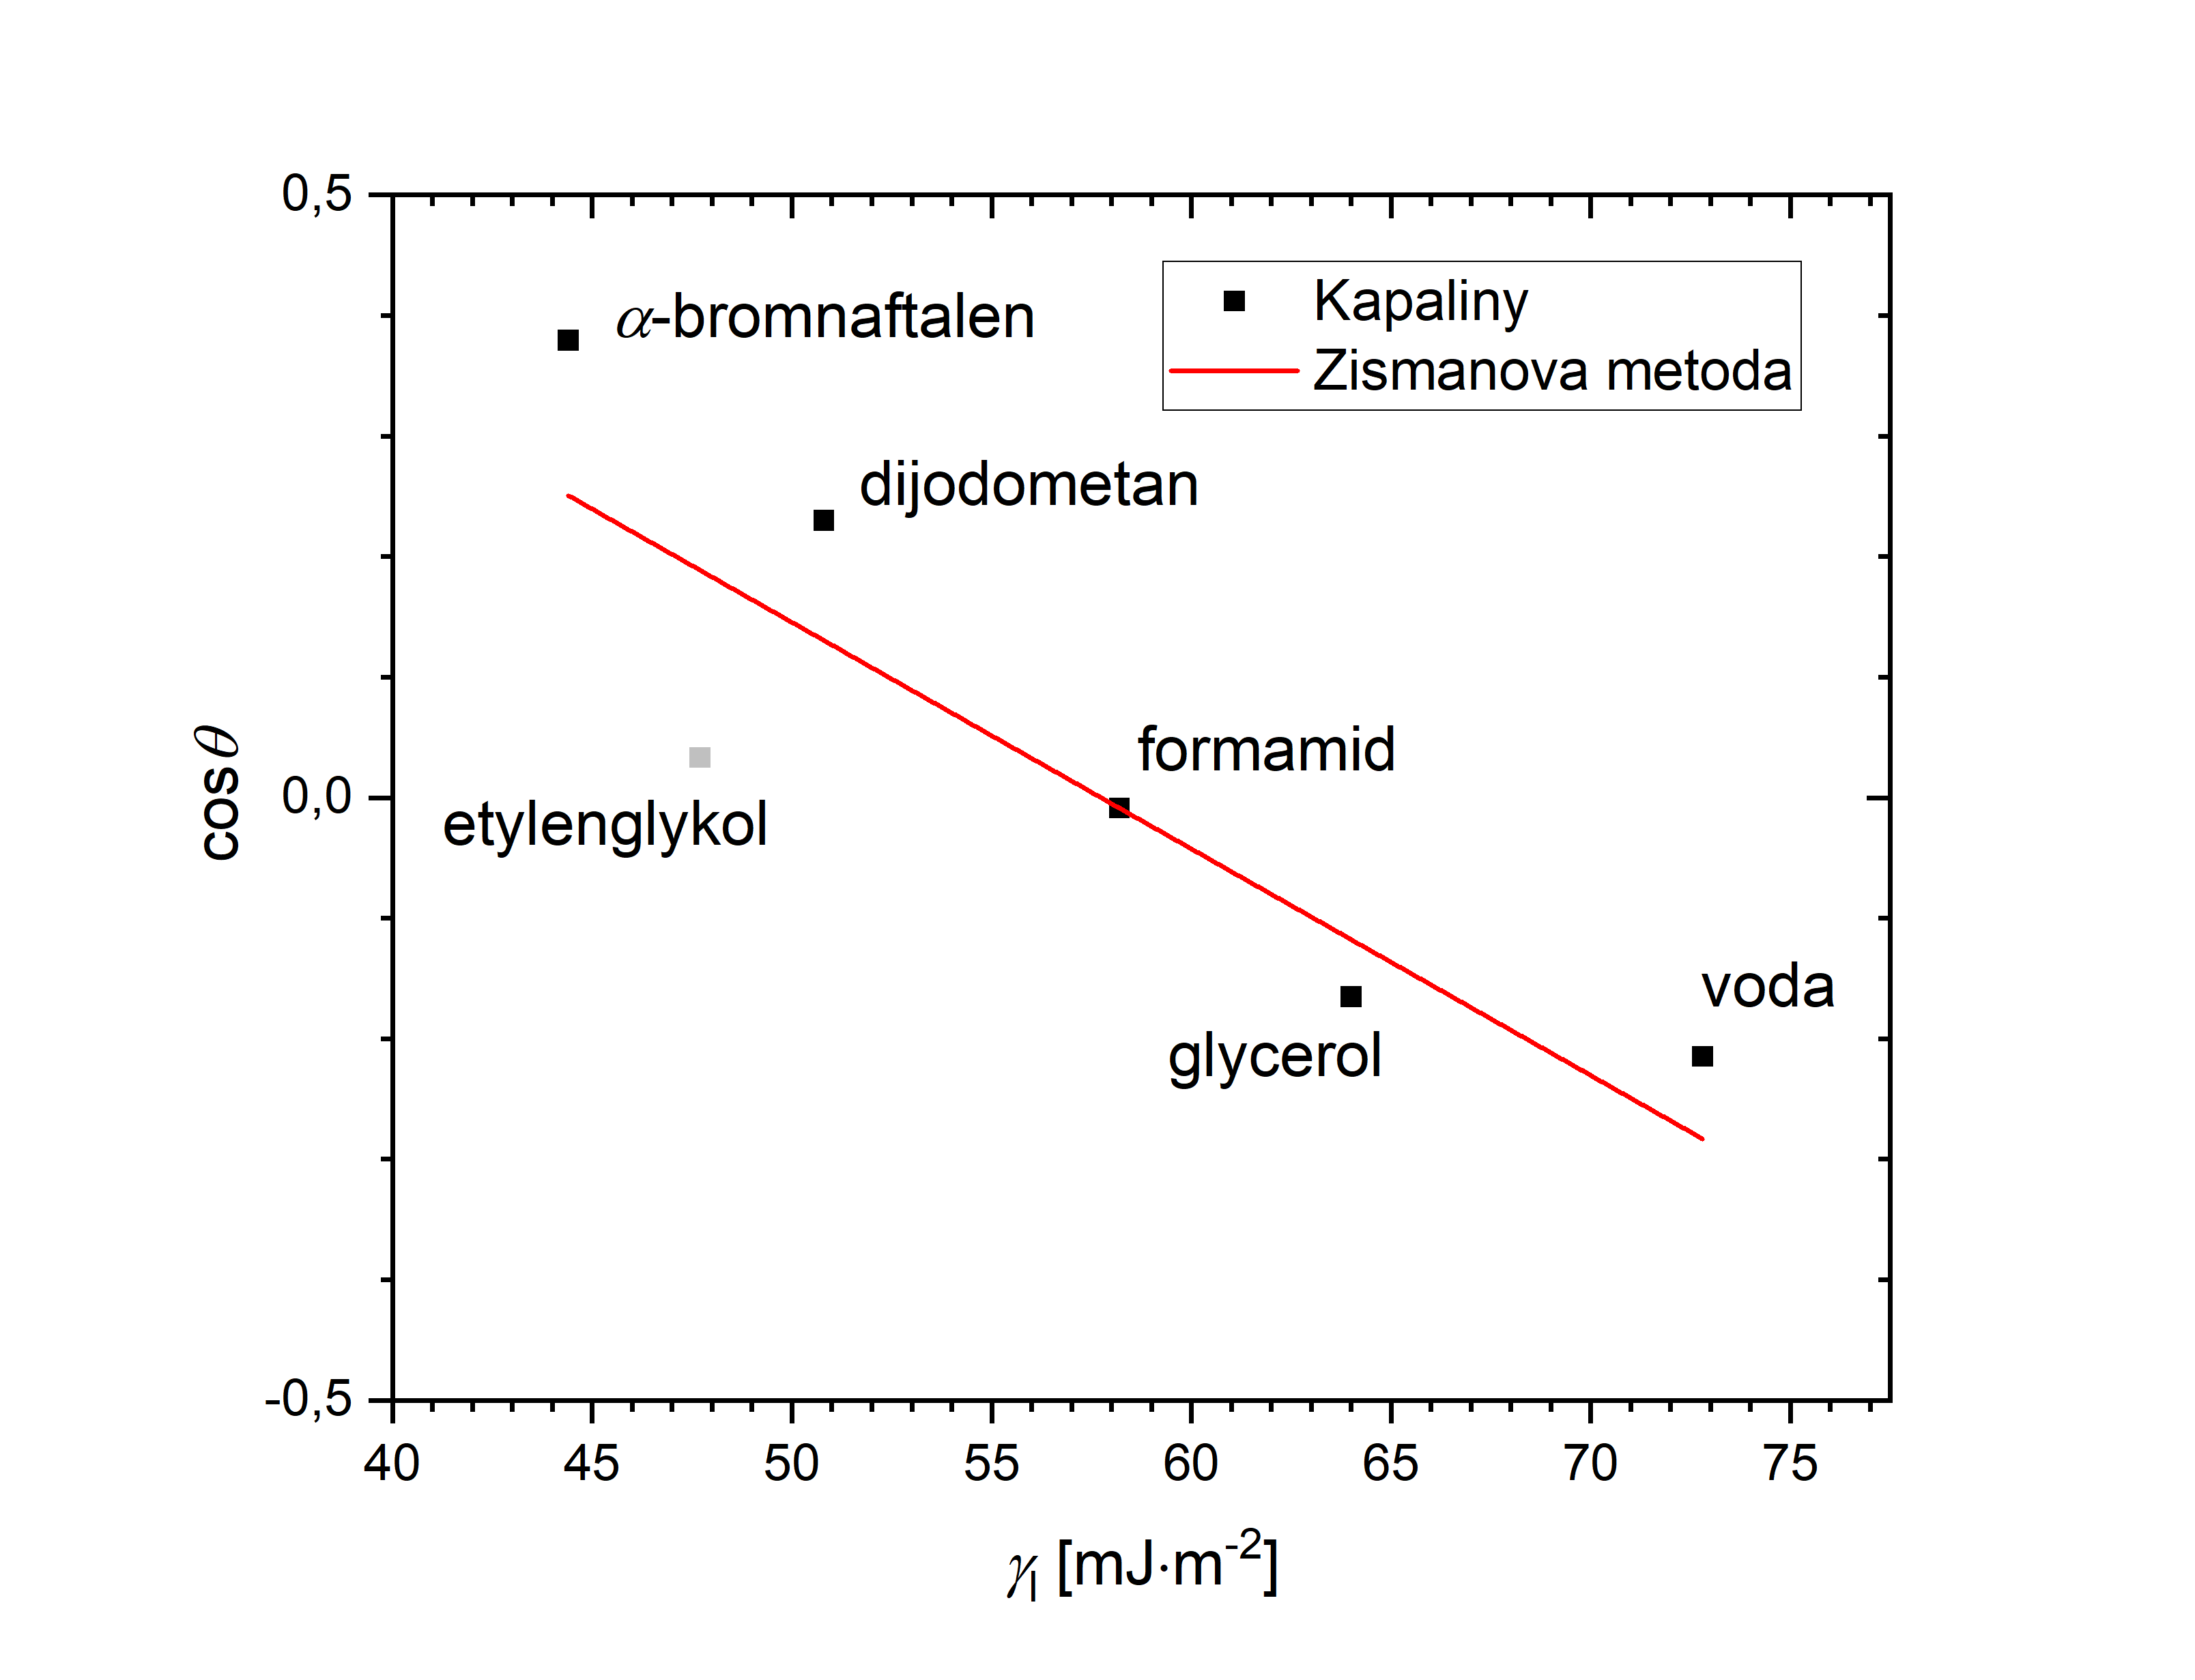
\includegraphics[width=130mm]{zisman.png}
	\caption{Závislost $\cos\theta = 
		f\left(\gamma_{\text{l}} \right)$ pro určení $\gamma_{\text{c}}$ 
		Zismanovou metodou.}
	\label{graph:zisman}
\end{figure}
\newpage
\subsection{Li-Neumann metoda}
\par Li-Neumann metoda je založená na stavové rovnici 
$W_\text{sl}=f(\gamma_{\text{lv}},\gamma_{\text{sv}})$. Výsledný tvar rovnice 
pro výpočet Li-Neumann metodou je
\begin{equation}
	\cos\theta = -1 + 
	2 {\left( \frac{\gamma_{\text{sv}}} {\gamma_{\text{lv}}} \right)}^{1/2} 
	\e^{-0,0001247(\gamma_{\text{lv}} - \gamma_{\text{sv}})^2}
\end{equation}

Software See System určil hodnotu povrchové energie teflonu pro každou 
kapalinu (tab.~\ref{table:LiNeumann}), jejich aritmetický průměr je 
$\gamma_{\text{c}} = (20,6\pm1,0)$\,\si{\milli\joule\per\meter\squared}.

\begin{table}[h]
	\caption{Softwarem určené povrchové energie teflonu pomocí Li-Neumann 
	metody.}
	\label{table:LiNeumann}
	\begin{tabular}{|c|c|}\hline
		kapalina  & Povrchová energie 
		$\gamma_{\text{c}}$\,[\si{\milli\joule\per\meter\squared}] \\ \hline
		destilovaná voda & $21,6 \pm 2,1$     \\
		etylenglykol     & $16,4 \pm 2,1$     \\
		dijodometan      & $23,3 \pm 2,1$     \\
		glycerol         & $18,7 \pm 3,5$     \\
		formamid         & $20,3 \pm 1,6$     \\
		$\alpha$-bromnaftalen & $23,5 \pm 1,4$\\ \hline
	\end{tabular}
\end{table}

\subsection{Kwok-Neumann metoda}
\par Pro Kwok-Neumann metodu, která stejně jako předchozí Li-Neumann metoda vychází ze stavové rovnice $W_\text{sl}=f(\gamma_{\text{lv}},\gamma_{\text{sv}})$, platí rovnice
\begin{equation}
	\cos\theta = -1 + 
	2 {\left(\frac{\gamma_{\text{sv}}}{\gamma_{\text{lv}}}\right)}^{1/2} 
	\left(1-0,0001057(\gamma_{\text{lv}} - \gamma_{\text{sv}})^2\right)
\end{equation}

Obdobným způsobem jako v předchozích případech software určil hodnotu povrchové 
energie teflonu pro každou kapalinu (tab.~\ref{table:KwokNeumann}), jejich 
aritmetický průměr je 
$\gamma_{\text{c}} = (20,3\pm1,0)$\,\si{\milli\joule\per\meter\squared}.

\begin{table}[h]
	\caption{Softwarem určené povrchové energie teflonu pomocí Kwok-Neumann 
	metody.}
	\label{table:KwokNeumann}
	\begin{tabular}{|c|c|}\hline
		kapalina  & Povrchová energie 
		$\gamma_{\text{c}}$\,[\si{\milli\joule\per\meter\squared}] \\ \hline
		destilovaná voda & $21,5 \pm 1,8$     \\
		etylenglykol     & $16,1 \pm 2,1$     \\
		dijodometan      & $22,9 \pm 2,3$     \\
		glycerol         & $18,4 \pm 3,0$     \\
		formamid         & $19,9 \pm 1,5$     \\
		$\alpha$-bromnaftalen & $23,2 \pm 1,6$\\ \hline
	\end{tabular}
\end{table}

\subsection{Wu metoda}
\par Následující tři modely jsou založeny na Fowkesovy teorii a jsou považovány 
za moderní modely. Fowkesova teorie bere v úvahu všechny síly, které působí 
mezi kapalinou a pevnou látkou 
\begin{equation}
\gamma = \gamma^\text{d} + \gamma^\text{p} +
\gamma^\text{h} + \gamma^\text{i} + \gamma^\text{ab} + ...
\end{equation}
\par Wu odvodil metodu kombinující harmonický a geometrický průměr. Tato metoda 
je vhodná pro vysoce energetické povrchy, pro teflon tedy také 
není vhodná. Povrchovou energii $\gamma_{\text{c}} = 
\gamma_{\text{s}}^{\text{d}} + \gamma_{\text{s}}^{\text{p}}$ určuje z rovnice
\begin{equation}
	\left(1+\cos\theta\right)\gamma_{\text{l}} = 
	4\left(\frac{\gamma_{\text{s}}^\text{d}\gamma_{\text{l}}^\text{d}}{\gamma_{\text{s}}^\text{d}
		+ \gamma_{\text{l}}^\text{d}} + 
	\frac{\gamma_{\text{s}}^\text{p}\gamma_{\text{l}}^\text{p}}{\gamma_{\text{s}}^\text{p}
		+ \gamma_{\text{l}}^\text{p}}\right)
\end{equation}
Software See System určil hodnotu povrchové energie teflonu pro každou 
kapalinu (tab.~\ref{table:Wu}), kde jejich aritmetický průměr je 
$\gamma_{\text{c}} = (15,0\pm1,6)$\,\si{\milli\joule\per\meter\squared}.

\begin{table}[h]
	\caption{Softwarem určené povrchové energie teflonu pomocí Wu metody.}
	\label{table:Wu}
	\begin{tabular}{|c|c|}\hline
		kapalina  & Povrchová energie 
		$\gamma_{\text{c}}$\,[\si{\milli\joule\per\meter\squared}] \\ \hline
		destilovaná voda & $11,2 \pm 1,8$     \\
		etylenglykol     & $12,8 \pm 2,1$     \\
		dijodometan      & $19,2 \pm 2,3$     \\
		glycerol         & $11,2 \pm 3,0$     \\
		formamid         & $14,2 \pm 1,5$     \\
		$\alpha$-bromnaftalen & $21,1 \pm 1,6$\\ \hline
	\end{tabular}
\end{table}

\subsection{Owens-Wendtova regresní metoda}
Rozšiřuje Fowkesovu teorii, kde interakční energie sil je vyjádřena jako 
geometrický střed polárních a disperzních komponent kapaliny a pevné látky. Po 
naměření kontaktního úhlu několika kapalin software určí povrchovou energii 
pomocí regresní metody:
\begin{equation}
	\frac{1+\cos\theta}{2}\frac{\gamma_{\text{l}}}{\sqrt{\gamma_{\text{l}}^\text{d}}}
	 = \sqrt{\gamma_{\text{s}}^\text{d}} + \sqrt{\gamma_{\text{s}}^\text{p}} 
	 \sqrt{\frac{\gamma_{\text{l}}^\text{p}}{\gamma_{\text{l}}^\text{d}}}
\end{equation}
\par Celková povrchová energie je $\gamma_{\text{c}} = (19,0 \pm 
3,1)$\,\si{\milli\joule\per\meter\squared}, přičemž software dokáže určit i 
složky povrchové energie -- Lifshitz Van der Waalsovu a acidobazickou: 
$\gamma^\text{LW} = (18,3\pm3,0)$\,\si{\milli\joule\per\meter\squared}, respektive
$\gamma^\text{AB}~=~(0,7~\pm~0,7)$\,\si{\milli\joule\per\meter\squared}


\subsection{Acidobazická regresní metoda}
\par Acidobazická metoda předpokládá, že celková povrchová energie je složena z 
Lifshitz Van der Waalsovy a acidobazické složky $\gamma_{\text{c}} = 
\gamma^\text{LW} + \gamma^\text{AB}$. Do acidobazické složky patři kovalentní, 
iontové a kovové síly, do Van der Waalsovy síly jsou zahrnuty coulombovské, 
indukční, disperzní a další. Určení povrchové energie z naměřených kontaktních 
úhlů $\theta$ probíhá regresní metodou:
%\begin{equation}
%	\gamma = \gamma^{\text{LW}} + \gamma^{\text{AB}}
%\end{equation}
%\begin{equation}
%	\gamma^{\text{AB}} = 2\sqrt{\gamma^+\gamma^-}
%\end{equation}
\begin{equation}
		\left(1+\cos\theta\right)\gamma_{\text{l}} = 
		2\left(\sqrt{\gamma_\text{l}^{\text{LW}}\gamma_\text{s}^{\text{LW}}} + 
		\sqrt{\gamma_\text{l}^{\text{+}}\gamma_\text{s}^{\text{-}}} + 
		\sqrt{\gamma_\text{l}^{\text{-}}\gamma_\text{s}^{\text{+}}}\right)
\end{equation}
\par Celková povrchová energie vypočítána softwarem $\gamma_{\text{c}} = (22,1 
\pm 
1,1)$\,\si{\milli\joule\per\meter\squared}. Lifshitz Van der Waalsova a 
acidobazická složka jsou rovny $\gamma^\text{LW} = 
(20,4\pm0,9)$\,\si{\milli\joule\per\meter\squared}, 
$\gamma^\text{AB} = (1,7\pm0,6)$\,\si{\milli\joule\per\meter\squared}

\subsection{Srovnání metod}
\par Na obr.~\ref{graph:srovnani} jsme vynesli srovnání metod včetně odchylek a 
tabulkové hodnoty $\gamma_{\text{c}} = 
20,0$\,\si{\milli\joule\per\meter\squared} \cite{napetiTeflon}. Sledujeme, že 
Zisman a Wu jsou nevhodné a nepřesné metody pro určení povrchové energie 
teflonu, zatímco ostatní metody jsou vyhovující, přičemž Li-Neumann a 
Kwok-Neumann jsou velmi přesné, v~případě, že nedošlo při měření k chybám 
uvedených v úvodní části.
\begin{figure}[h!]
	\centering
	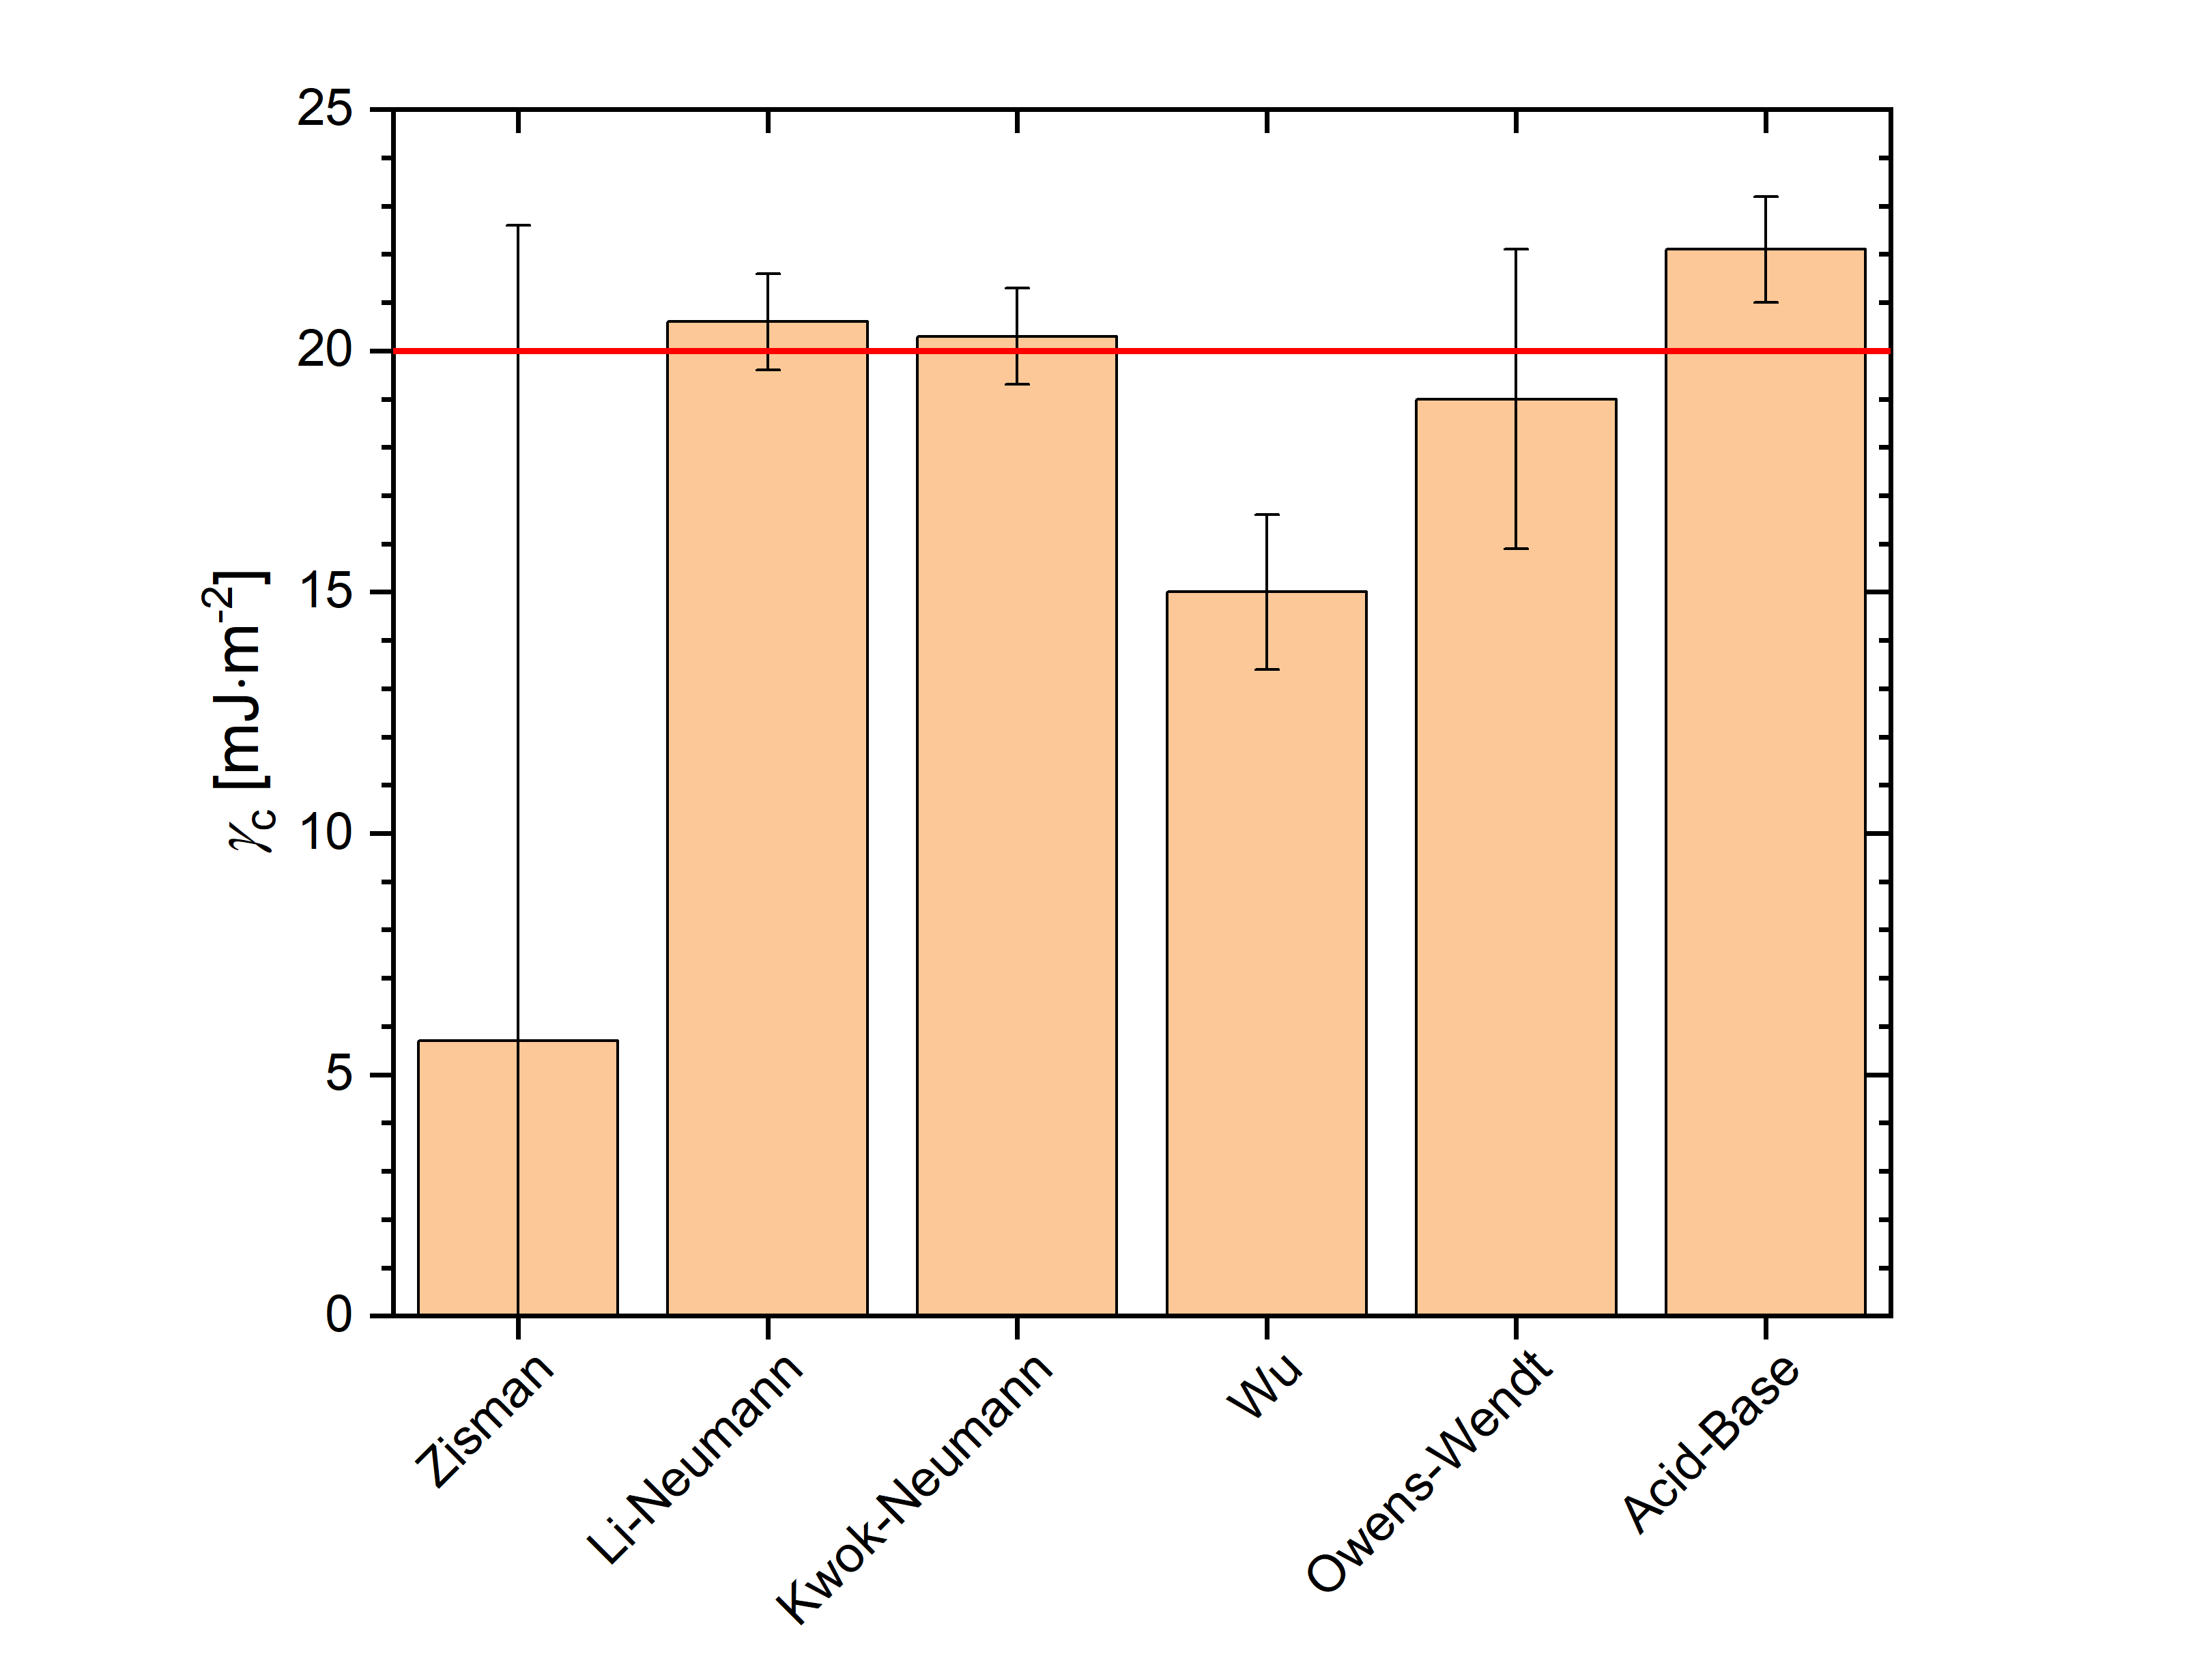
\includegraphics[width=130mm]{srovnani.png}
	\caption{Srovnání výsledků jednotlivých metod určení povrchové energie 
	teflonu $\gamma_{\text{c}}$, červená vodorovná čára značí tabulkovou 
	hodnotu pro teflon $\gamma_{\text{c}} = 
	20,0$\,\si{\milli\joule\per\meter\squared} \cite{napetiTeflon}.}
	\label{graph:srovnani}
\end{figure}


\section{Závěr}
V této úloze jsme se zabývali měřením povrchové energie  $\gamma_{\text{c}}$. 
Konkrétně jsme měřili povrchovou energii teflonu kapkovou metodou pomocí 
přístroje See System. Pro výpočet povrchové energie jsme použili několik metod, 
vstupními parametry pro výslednou hodnotu byly námi naměřené kontaktní úhly 
šesti různých kapalin. První metodou byla Zismanova. Pro ni jsme ke srovnání s 
hodnotou $\gamma_{\text{c}}~=~(5,7~\pm~16,9)$\,\si{\milli\joule\per\meter\squared} získanou ze softwaru See 
Systemu nafitovali danou závislost i ručně, přičemž nám vyšlo 
$\gamma_{\text{c}} = (4,5\pm11,5)$\,\si{\milli\joule\per\meter\squared}. Obě 
hodnoty se v rámci chyby shodují, ta je ovšem příliš velká a~tato metoda se 
tedy jeví jako nevhodná. Z Li-Neumannovy metody vychází $\gamma_{\text{c}} = 
(20,6\pm1,0)$\,\si{\milli\joule\per\meter\squared}. Kwok-Neumannova metoda dává 
v rámci chyby stejný výsledek $\gamma_{\text{c}} = 
(20,3\pm1,0)$\,\si{\milli\joule\per\meter\squared}, což je očekávané, protože 
obě metody vychází ze stejné stavové rovnice. Zároveň odpovídají tabulkové 
hodnotě $\gamma_{\text{c}} = 20$\,\si{\milli\joule\per\meter\squared} 
\cite{napetiTeflon}. Výpočtem z Wu metody jsme získali hodnotu 
$\gamma_{\text{c}} = (15,0\pm1,6)$\,\si{\milli\joule\per\meter\squared}, což 
ukazuje, že tato metoda je nevhodná pro měření povrchů s nízkou energií. 
Owens-Wendtova regresní metoda dává hodnotu $\gamma_{\text{c}} = 
(19,0\pm3,1)$\,\si{\milli\joule\per\meter\squared} a rozložení na Lifshitz Van 
der Waalsovu $\gamma^\text{LW} = 
(18,3\pm3,0)$\,\si{\milli\joule\per\meter\squared} a acidobazickou složku
$\gamma^\text{AB} = (0,7\pm0,7)$\,\si{\milli\joule\per\meter\squared}. 
Acidobazická metoda dává nejvyšší hodnotu ze všech metod $\gamma_{\text{c}} = 
(22,1\pm1,1)$\,\si{\milli\joule\per\meter\squared} a její složky 
$\gamma^\text{LW} = (20,4\pm0,9)$\,\si{\milli\joule\per\meter\squared}, 
$\gamma^\text{AB} = (1,7\pm0,6)$\,\si{\milli\joule\per\meter\squared}.
\newpage
\begin{thebibliography}{10}
	\bibitem{napetiKapalin} {\textit{Surface tension values of some common test 
	liquids for surface energy analysis} [online]. Dostupné z: 
	http://www.surface-tension.de/}
	
	\bibitem{napetiTeflon} {\textit{Solid surface energy data for common polymers} [online]. Dostupné z: http://www.surface-tension.de/solid-surface-energy.htm}

	
\end{thebibliography}

\end{document}
